\chapter{Content Retrieval Infrastructure}
\label{content_retrieval}

\section{Motivation}

Most of the applications today that need to deliver content reliably
use TCP as the transport layer protocol. The motivating example in our
case is the world wide web. TCP relies on communication from end-hosts
to provide reliable content delivery. Relying on end hosts rather than
the network for the reliable delivery information gives TCP the
advantage that no explicit network layer feedback is needed to
reliably transport content. This goes in accordance with the
philosophy of a dumb network and smart ends and the end-to-end
principle.

However, the rise of information centric networking shifts the focus
from hosts to content. That poses us with the challenge of redesigning
reliable transport for content centric architectures. The solutions
that have been proposed to rely on client applications to fetch
individual packets belonging to a object reliably. This approach of
one-way reliability loses on important congestion control information
that the content provider (a router cache or the original publisher)
could have received from the client. An example of such information
could be the congestion window size.

We, therefore, take a different approach to solve the problem of
reliable transport of content chunks. We use coexisting content and
service principles in XIA to allow us to apply TCP like congestion
control and reliability approach to content centric networks. The
content principle helps in locating the content and the service
principle helps in delivering the content. We show that this approach
of delivering content-over-service does not change the semantics of
use and still allows both the publisher and the client to
participate in a reliable content transport session resulting in a
more efficient reliable content transport for content centric
architectures.

\section{Design Goals}

As we have seen in the last chapters, XIA does not disregard the fact
that the first class principle the world is moving towards is
content. At the same time it allows for presence of multiple such
principles simultaneously. In the new content retrieval infrastructure
we aim to leverage the coexistence of “services” and “content”
principles. We aim to solve problem the problem of reliable transport
of content for content centric networks using the coexisting service
and content principles.

While solving other problems, we aim to ensure that the benefits
expected out of an information-centric architecture are still
preserved. So, ICN features such as on path caching, content based
routing should remain as they are.

Also, we envision that the cache on routers could extend in multiple
dimensions. For example, cache could choose to store content at a
remote location rather than in its local storage. Content eviction
policies might change over time.  Thus, it is important that the
system we design is extensible in all the ways possible.

\section{Design Overview}

\begin{figure}
  \begin{center}
    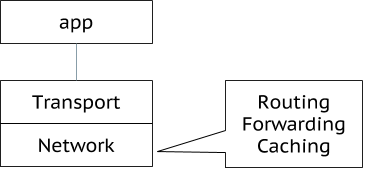
\includegraphics[scale = 0.75]{old_stack}
    \caption{Old Network Stack for Content Delivery Architecture}
    \label{fig:old_stack}
  \end{center}
\end{figure}

\begin{figure}
  \begin{center}
    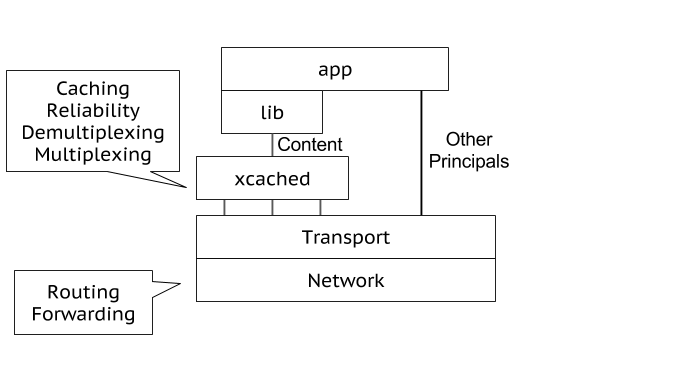
\includegraphics[scale = 0.75]{new_stack}
    \caption{New Network Stack for Content Delivery Architecture}
    \label{fig:new_stack}
  \end{center}
\end{figure}
As we have seen in chapter \ref{chap:ccnxia}, cacheable content is
addressed using CIDs. CID principle puts no limit on the size of the
content chunk. Although desirable, this requirement implies that some
applications will need the ability to transmit and fetch content
reliably. How does it affect our design?  Let’s look at where various
functionalities are implemented in XIA’s network stack. The old
network stack for content delivery architecture is outlined in
\ref{fig:old_stack}. Reliable transport service (streaming sockets) is
implemented at transport layer in this stack. In order to transmit
content reliably, we need a way to use reliable transport
service. Therefore in our new design, we implement content delivery
infrastructure primarily in an application while keeping content based
routing as it is. The new network stack and the functionality split is
as shown in \ref{fig:new_stack}.

The fact that caching is moved to an application gives us following
advantages:
\begin{itemize}
\item{Extensibility}
\item{Easy access to reliable transport API}
\end{itemize}

We define a new application level entity called Xcache Daemon(xcached)
that takes the responsibility of caching and serving content chunks.
Xcached receives requests from client applications and translates them
into socket calls as shown in table \ref{tab:apis}. Xcached also takes
care of multiplexing and demultiplexing of content requests and
responses to and from various connected content applications.

\section{Xcached Architecture}

Xcached is the center of all CID (as well as nCID as we will see in
the later chapters) operations. So, it is important that it does not
become the bottleneck in the content delivery infrastructure. It
essentially means that xcached should not starve applications, it
should process requests fairly and it should be performant. In this
section we will look closely at the xcached daemon - how it has been
architected and what are some of its extensibility characteristics.

\begin{figure}
  \begin{center}
    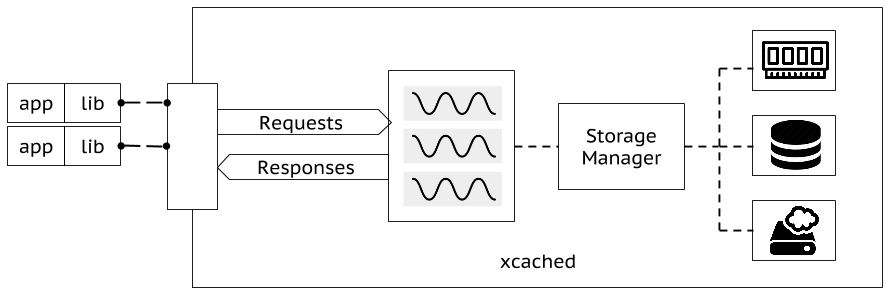
\includegraphics[scale = 0.45]{xcached_arch}
    \caption{Xcached Architecture}
    \label{fig:xcached_arch}
  \end{center}
\end{figure}
Xcached is a mutli-threaded program that follows worker thread pool
model in which the application facing controller puts the arrived
requests in a queue and worker threads dequeue and do the work as and
when convenient. \ref{fig:xcached_arch} shows the various modules in
the xcache daemon.

\subsection{XcacheLib}
In order to hide communication details from the application, we have
built a library that exposes the required APIs to the content
applications. These APIs are described in greater details in section
\ref{sec:apis}.

\subsection{The controller}
The controller is the application facing front end which takes
requests from the XcacheLib. The communication between the controller and
XcacheLib is over UNIX domain sockets. We use google-protobuf to parse
and unparse the requests to and from the controller. It is possible that
applications request for content that is cached locally. The controller
processes such requests in fast-path. I.e. It sends back the response
to the application quickly. All the other requests which cannot be
processed in the fast path are put in the requests queue. These
requests are processed at some time in future by one of threads in the
thread pool.

\subsection{Thread Pool}
\begin{table}
  \begin{center}
    \begin{tabular}
      { p{1in} | p{2.5in} | cp{0.5in} |}
      Job & Details & No. of threads \\
      \hline
      Content Publish / Fetch & Storing content published by applications or fetching content from a remote source &  Arbitrary\\
      \hline
      Content Eviction on Timeout & Content objects that get cached have a associated time-to-live period. This is the time period after which content object should become unavailable. & One \\
      \hline
      Opportunistic Caching & Opportunistic caching of content chunks
      by in-network devices & One\\
    \end{tabular}
    \caption{Jobs performed by threads in xcached}
  \end{center}
  \label{tab:threads}
\end{table}
Xcached thread pool consists of a set of worker threads, number of
which can be configured at xcached startup. The thread pool consists
of threads that perform one of the tasks shown in table
\ref{tab:threads}.
\subsection{Content Stores}
Different content systems have different characteristics: RAM allows
fast retrieval of data but has limited size. Disk is slower than RAM
store but can hold a lot more content. Thus storing content in RAM
might be more desirable for use cases that need only smaller chunks
whereas use cases that need to store big content chunks might prefer
to store content on Disk rather than in RAM. In order to support these
varying use cases, Xcached supports multiple different content storage
methods. By default, it supports storing content in RAM, on disk and
on a network attached storage device. Also, it is possible to compile
new storage methods with xcached. Implementing a new storage method is
as simple as extending following class and implementing the member
methods.

{
  \setstretch{1.0}
\begin{verbatim}
class xcache_content_store {
        virtual store();
        virtual get();
}
\end{verbatim}
}

\subsection{Storage Manager}
Since xcached has different storage methods, it is possible to
organize content objects across these stores in different ways to
serve different use-cases. Possible content placement policies could
be round-robin, popularity based or size based. We implement a simple
content placement policy which places content in RAM store until it’s
full and then moves subsequent content to the disk store.

\subsection{Content Eviction}
If possible content stores run out of space, content must be evicted
to make space for new incoming content. Content eviction policies
govern which content chunks should be evicted on such an event from a
particular content store. The content eviction policy that Xcache
supports is LRU (Least recently used). Just like content stores, new
content eviction policies can be compiled with xcache and associated
with the content stores. Implementing new content eviction policies is
just as simple as extending and implementing following class.

{
  \setstretch{1.0}
\begin{verbatim}
class xcache_eviction_policy {
        virtual store();
        virtual get();
        virtual remove();
        virtual evict();
}
\end{verbatim}
}


\section {Design Details}

Xcached has three types of interfaces with the transport layer. In
order to understand these interfaces better let's take a closer look
at three network components that interact with XcacheD.

\subsection{Content Server}
Xcached acts as a content server on the publisher's end as well as
when the in-network cache delivers content to the client. On receipt
of content requests, the daemon needs to know what content is being
requested. We define a new type of transport socket called ``content
server'' socket which allows daemon to bind to all the content
connections. This socket allows xcached to know for what content the
request was received.  The content server socket needs to do two
unusual tasks which are significantly different from normal server
sockets.

\subsubsection{Bind(Content *)}
Since content server needs to listen to all incoming content
request, it needs to bind to all content addresses that the provider
has with it. Thus we need a notion of \texttt{Bind(Content *)}.

\subsubsection{AcceptAs(MyAddress)}
As the server side socket has been bound to many addresses, when an
incoming request is received, the xcached needs to know for which
address the request was received. In other words, the server needs a
way to know what address is the source address for packets going out
of it. Thus we define a new \texttt{AcceptAs} call that tells xcached
for which content the request was received.

\subsection{Content Client}
The main responsibility of client side xcached is to establish a
reliable transport session with a content provider and fetch content
reliably. The content provider can be an in-network cache or it can be
the end publisher. So, xcached's client side socket ``connects'' with a
content provider and fetches the content. In other words, xcached's
client socket ``connects'' with content rather than a ``service''.

\subsection{Opportunistic Caching}
The last context in which xcached comes into picture is opportunistic
caching. When content providers serve content to clients over a
reliable transport session, in-network devices need to intercept and
cache content packets as they are traveling through them. The third
interface that xcached has with the network allows xcached to sniff
content packets flowing through it. We call this socket a content raw
socket.

\begin{table}
  \begin{center}
    \begin{tabular}
      {| c | c |}
      API & What xcache does \\
      \hline
      XputChunk & StoreContent(), XaddRoute() \\
      XgetChunk & Xconnect(CID Dag), Xrecv() \\
    \end{tabular}
    \label{tab:apis}
    \caption{API Expansion}
  \end{center}
\end{table}
\section{End to End Example}

We have seen at high level how we moved caching and content serving
functionality to xcached application. In this section we will walk
through a detailed end to end example and see how clients establish
a reliable transport session with a publisher and how intermediate
caches cache the packets flowing through them.

\subsection{Step 1: \texttt{XputChunk(Content)}}
The whole story starts with the publisher putting the content objects
in the local cache (xcached) and publishing routes to these content
objects. This lets the network know that unless cached at a better
location, all the incoming requests for this content should be
forwarded to this host. The end publisher publishes the chunk with the
DAG address as shown in \ref{fig:cid_dag_publisher}.

\begin{figure}
  \begin{center}
    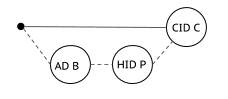
\includegraphics[scale = 0.75]{cid_dag_publisher}
    \caption{CID Dag Publisher}
    \label{fig:cid_dag_publisher}
  \end{center}
\end{figure}
\subsection{Step 2: \texttt{XgetChunk(CID\_Dag)}}
\begin{itemize}
\item{Client application calls \texttt{XgetChunk} with the desired DAG
  address as the argument. This call lets the xcached know that a client
  application is interested in fetching content pointed to by the
  DAG.}
\item{Xcached tries to establish the reliable transport session with
  one of the many network entities who can serve the content by calling
  \texttt{Xconnect(CID-Dag)}. This \texttt{Xconnect(CID-Dag)} call
  serves two purposes: It acts as a content request as well the first
  packet of three-way handshake of the reliable transport session
  (SYN).}
\item{Any network device that has the content chunk cached, accepts
  the GET / SYN packet and in effect tells xcached that there is a
  content request and it is the first packet of the reliable transport
  session.}
\item{Call to \texttt{XacceptAs} made by xcached then returns with the
  address of content that was requested by the client. The return of
  \texttt{XaccetAs} also means that the three-way handshake was
  completed by the xcached that provides the content.}
\end{itemize}
\subsection{Addresses}
The SYN packet that xcached on the content provider received, has the
source address that looks like address in \ref{fig:dag_syn_source}.

\begin{figure}
  \begin{center}
    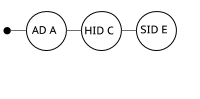
\includegraphics[scale = 0.75]{dag_syn_source}
    \caption{SYN Source Address}
    \label{fig:dag_syn_source}
  \end{center}
\end{figure}
The SID in the source address represents the ephemeral reliable
transport endpoint that xcached on client had created. This address
acts as a way back to the client. Content server socket completes
the three way handshake by accepting the connection with source
address as in \ref{fig:source_cid_addr}.
\begin{figure}
  \begin{center}
    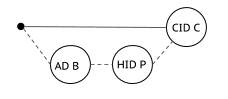
\includegraphics[scale = 0.75]{cid_dag_publisher}
    \caption{CID Dag Publisher}
    \label{fig:source_cid_addr}
  \end{center}
\end{figure}
Once the connection has been accepted, content provider serves the
content over the established reliable transport session.

\subsection{Opportunistic Caching}
The challenge in opportunistically caching the content objects is that
the xcached on the in-network cache is not an active participant in
the reliable transport session. We solve the problem of opportunistic
caching by forwarding all the content packets to xcached and then
reassembling the chunk by peeking into transport header. Following are
the steps that take place on the intermediate cache when content
object is to be cached.
\begin{itemize}
\item {While content is being served from the content provider to content
client, it gets caught by the CID raw sockets on Xcached's running
on intermediate network devices. The CID raw socket forwards all the
packets which have the primary intent as CID to the xcached
running.}
\item {Looking at the first packet in the transport session (SYN/ACK),
  the forwarding engine needs to know if the content object should be
  cached or not. The logic for this policy is implemented in
  xcached. Based on the policy, xcached takes a decision and either
  sends ``Yes, cache'' or ``No, don't cache'' decision to the
  forwarding engine}
\item {Packets belonging to all content chunks for which the policy
  decision is ``Yes, cache'' are forwarded to xcached.}
\item {Xcached peeks into the transport header and reassembles a
  content object. Once reassembled, now that particular xcached also
  acts as the content provider for the chunk.}
\end{itemize}


\section{API Details}
\label{sec:apis}
With the movement of caching and content handling to xcache
application, we also redefined the application interfaces for
publishing and fetching content over XIA. The application is not
responsible for establishing the reliable transport session. Xcached
does it on behalf of the application. This simplifies the application
design and also gives the xcached the ability to cache content that
was requested by the application. In this section, we will go over the
APIs that XcacheLib exposes to the content applications and see an
example of a sample content publisher as well as a client application.
\begin{itemize}
\item{\texttt{int XcacheHandleInit(XcacheHandle *h)}} - Creates a
  connection with \texttt{xcached} and fills in the opaque structure
  \texttt{XcacheHandle}. \texttt{XcacheHandle} acts as a context for
  the rest of the APIs.
\item{\texttt{int XcacheHandleDestroy(XcacheHandle *h)}} - Destroys
  the the handle created by the call
  \texttt{XcacheHandleInit}. Applications that call
  \texttt{XcacheHandleInit} must call \texttt{XcacheHandleDestroy}.
\item{\texttt{int XfetchChunk(XcacheHandle *h, void *buf, size\_t buflen,
    int flags, sockaddr\_x *addr, socklen\_t addrlen)}} - This
  function lets applications fetch content chunk that has the DAG
  address \texttt{addr} of length \texttt{addrlen}. The Xcache context
  \texttt{h} must be initialized by calling function
  \texttt{XcacheHandleInit}.

\item{\texttt{int XputChunk(XcacheHandle *h, const void *data, size\_t
  length, sockaddr\_x *addr)}} - \texttt{XputChunk} allows
  applications to publish chunks to the network. A call to
  \texttt{XputChunk} publishes a chunk which has data pointed to by
  \texttt{data} and of length \texttt{length}. The address of the
  published chunk is returned in the address \texttt{addr}.
\item{\texttt{int XregisterNotif(int event, void (*func)(XcacheHandle
    *, int event, sockaddr\_x *addr, socklen\_t addrlen))}} - Xcache
  allows applications to listen for certain
  ``notifications''. Examples of these notifications include chunk
  eviction notification, chunk arrival notification. A call to
  \texttt{XregisterNotif} registers a handler for a particular
  notification. Applications can either spawn a separate thread for
  handling notifications by calling \texttt{XlaunchNotifThread} or
  they can look for received notifications by checking received data
  on socket returned by \texttt{XgetNotifSocket} and calling
  \texttt{XprocessNotif} if appropriate.
\item{\texttt{int XlaunchNotifThread(XcacheHandle *h)}} - This
  function launches a notification listener thread. If
  \texttt{xcached} sends a notification on notification socket, the
  function calls registered handlers if appropriate.
\item{\texttt{int XgetNotifSocket(XcacheHandle *h)}} - This function
  returns the socket on which \texttt{xcached} sends back the
  notifications.
\item{\texttt{int XprocessNotif(XcacheHandle *h)}} - If the
  \texttt{xcached} notifcation socket has any incoming data,
  applications can call \texttt{XprocessNotif} to invoke the
  registered handlers.
\end{itemize}

\section{Sample Applications}
In this section, we will see how applications can use above mentioned
APIs in their code. Section \ref{sec:content_server_app} shows a
self-explanatory example of a content server application. Whereas,
section \ref{sec:content_client_app} shows a self-explanatory example
of a content client application.

\subsection{Content Server Application}
\label{sec:content_server_app}
      {
        \setstretch{1.0}
\begin{verbatim}
  int main(void) {
    XcacheHandle xcache;
    sockaddr_x info;
    ...
    XcacheHandleInit(&xcache);
    ...
    XputChunk(&xcache, data, datalen, 512, &info);
    ...
    XdetroyChunk(&xcache);
  }
\end{verbatim}
      }

\subsection{Content Client Application}
\label{sec:content_client_app}
      {
        \setstretch{1.0}
\begin{verbatim}
  int main(void) {
    XcacheHandle xcache;
    sockaddr_x info;
    ...
    XcacheHandleInit(&xcache);
    ...
    XfetchChunk(&xcache, buf, 1024, XCF_BLOCK, &info, sizeof(sockaddr_x));
    ...
    XdetroyChunk(&xcache);
  }
\end{verbatim}
}
\section{Conclusion}
In this chapter, we saw how we moved content caching and serving to an
application daemon \texttt{xcached}. In contrast to the old design, we
used reliable transport to deliver content. We then looked at the new
API and how we can use it to write content applications in XIA.
